\begin{problema}
        Sea $S_n=X_1+\cdots+X_n$ una caminata aleatoria con saltos $X_i\in \{-1,0,1,\ldots\}$. 
        Sea $C_p$ una variable aleatoria geom\'etrica de par\'ametro $p$ independiente de $S$ y definimos 
        
        \begin{align}
            M_p=-\min_{n\leq C_p} S_n. 
        \end{align}\par\null
        
        El objetivo del ejercicio es determinar la distribuci\'on de $M_p$.\par\null

        (A las caminatas aleatorias como $S$ se les ha denominado Skip-free random walks Para aplicaciones de este tipo 
        de procesos, ver \cite{MR1978607}. Tambi\'en aparecen en el estudio de Procesos Galton-Watson. 
        Este ejercicio es el resultado b\'asico del estudio de sus extremos, denominado teor\'ia de fluctuaciones.)

    \begin{enumerate}
        \item[(i)]  [\ref{problema2_1:inciso1}]
                    Sea
                    
                    \begin{align}
                        g(\lambda)=E(e^{- \lambda X_1}).
                    \end{align} 
                    
                    Pruebe que $g(\lambda)\in (0,\infty)$ y que
                    
                    \begin{align}
                        M_n=e^{-\lambda S_n}g(\lambda)^{-n},n\geq 0
                    \end{align}
                    
                    es una martingala.
        
        \item[(ii)] [\ref{problema2_1:inciso2}]
                    Pruebe que $g$ es log-convexa al aplicar la desigualdad de H\"older. Pruebe que si $P(X_1=-1)>0$ 
                    (hip\'otesis que se utilizar\'a desde ahora) 
                    entonces $g(\lambda)\to\infty$ conforme $\lambda\to\infty$. Utilice esta informaci\'on para esbozar la gr\'afica de $g$. 
                    Defina $ f(s)=\inf \{ \lambda>0:g(\lambda)^{-1} < s\} $. Note que $1/g\circ f=Id$ en $(0,1)$. Pruebe que si $g(\lambda)>1$, 
                    la martingala $M$ es acotada hasta el tiempo de arribo de $S$ a $-k$ dado por 
                    
                    \begin{align}
                        T_k =\min \{n\in\na:S_n=-k\} 
                    \end{align}
                    
                    (donde se utiliza la convenci\'on $\inf\emptyset=\infty$ ). Aplique el teorema de muestreo opcional de Doob para mostrar que 
                    
                    \begin{align}
                        E(s^{T_k})=e^{-k f(s)}.
                    \end{align}
                    
                    Justifique MUY bien por qu\'e la f\'ormula es válida aún cuando $T_k$ puede tomar el valor $\infty$ 
                    y deduzca que de hecho $\p (T_k=\infty)=0$.
                        
        \item[(iii)] [\ref{problema2_1:inciso3}]
                    Argumente que
        
                    \begin{align}
                        P(M_p\geq n)=P(T_n\leq C_p)=E((1-p)^{T_n})
                    \end{align}
                    
                    para demostrar que $M_p$ tiene distribuci\'on geom\'etrica de par\'ametro $1-e^{-f(1-p)}$.
                    
        \item[(iv)] [\ref{problema2_1:inciso4}]
                    Tome el límite conforme $p\to 0$ para mostrar que la variable aleatoria 
                    \begin{align}
                        M=-\min_{n\geq 0}S_n
                    \end{align}
                    tiene una distribuci\'on geom\'etrica de par\'ametro $1-e^{-f(1)}$. Interprete esto cuando $f(1)=0$.
    \end{enumerate}

        \defin{Categor\'ias:} Caminatas aleatorias, muestreo opcional, fluctuaciones.
\end{problema}


\begin{proof}
    \subsection{Inciso (i)}     \label{problema2_1:inciso1}
    \emph{
    Sea
        \begin{align}
                g(\lambda)=E(e^{- \lambda X_1}).
        \end{align} 
    Pruebe que 
        \begin{align}
                g(\lambda)    &\in (0,\infty)\label{problema2_1:parte1}
        \end{align}        
    y que
        \begin{align}
                M_n=e^{-\lambda S_n}g(\lambda)^{-n},n\geq 0
        \end{align}
    es una martingala.\\
}
    
    Para probar \eqref{problema2_1:parte1} notemos que
    \begin{align}
        e^x > 0 \;\; \forall x \in \R.
    \end{align}
    por lo tanto
    \begin{align}
        e^{-\lambda X_1} > 0
    \end{align}
    y entonces
    \begin{align}
        \E(e^{-\lambda X_1}) >\E(0) = 0
    \end{align}

    Falta ver que $\E(e^{-\lambda X_1})$ está acotada. Recordemos que $e^x$ es creciente y por lo tanto
    \begin{align}
        X_1                &\geq     -1                       & \Rightarrow\\
        1                  &\geq     - X_1                    & \Rightarrow\\
        \lambda            &\geq     - \lambda X_1            & \Rightarrow\\
        e^{\lambda}        &\geq     e^{- \lambda X_1}        & \Rightarrow\\
        \E(e^{\lambda})    &\geq     \E(e^{- \lambda X_1})
    \end{align}
    
    Pero $\E(e^{\lambda}) = e^{\lambda}$. Y por lo tanto
    
    \begin{align}
        e^{\lambda} \geq  \E(e^{- \lambda X_1})
    \end{align}    
    
    Entonces $0 < \E(e^{-\lambda X_1}) < \infty$, y con esto queda demostrado \eqref{problema2_1:parte1}.
    
    Probemos ahora que $(M_n)_{n \in \N}$ es martingala.
    
    \begin{itemize}
        \item 
            Veamos que $M_n$ es $\F_n$-medible.\\
            
            Para esto, recordemos que si $\G$ es una $\sigma$-algebra, $f$ es $\G$-medible y $g$ es continua
            con la topología usual de $\R$ entonces $g \circ f$ es $\G$-medible.\\
            
            $S_n$ es $\F_n$-medible. Multiplicar por constantes es función continua. Dividir entre constantes 
            es función continua. La función exponencial es continua. Y por lo tanto $M_n=e^{-\lambda S_n}g(\lambda)^{-n}$ 
            es composición de funciones continuas con $S_n$. De donde $M_n$ es $F_n$-medible.\\
         
        \item 
            Ahora veamos que $M_n \in L_1$.\\
            
            De la misma demostración que dimos para probar la primera parte, se sigue 
            que $0 < e^{-\lambda X_n} < \infty$ y que $e^{-\lambda X_n} \in \N$ para toda $n \in \N$. Por lo tanto
            
            \begin{align}
                M_n         &=      e^{-\lambda S_n}g(\lambda)^{-n} \\
                            &=      \prod_{1 \leq i \leq n} e^{-\lambda X_i} g(\lambda)^{-n}. 
            \end{align}
            
            Entonces, $M_n$ es producto finito de funciones en $L_1$, de donde tenemos que $M_n \in L_1$.
    \end{itemize}
    \newpage
    
    \subsection{Inciso (ii)}    \label{problema2_1:inciso2} 
    \emph{
    Pruebe que $g$ es $\log$-convexa al aplicar la desigualdad de H\"older. Pruebe que si $P(X_1=-1)>0$ (hip\'otesis que se utilizar\'a desde ahora) 
    entonces $g(\lambda)\to\infty$ conforme $\lambda\to\infty$. Utilice esta informaci\'on para esbozar la gr\'afica de $g$. 
    Defina $ f(s)=\inf \{ \lambda>0:g(\lambda)^{-1} < s\} $. Note que $1/g\circ f=Id$ en $(0,1)$. Pruebe que si $g(\lambda)>1$, 
    la martingala $M$ es acotada hasta el tiempo de arribo de $S$ a $-k$ dado por 
    \null
    \begin{align}
        T_k =\min \{n\in\na:S_n=-k\} 
    \end{align}
    \null
    (donde se utiliza la convenci\'on $\inf\emptyset=\infty$ ). Aplique el teorema de muestreo opcional de Doob para mostrar que 
    \null
    \begin{align}
        E(s^{T_k})=e^{-k f(s)}.
    \end{align}
    \null
    Justifique MUY bien por qu\'e la f\'ormula es válida aún cuando $T_k$ puede tomar el valor $\infty$ y deduzca que de hecho 
    $\p (T_k=\infty)=0$.
}
\afterstatement
    Primero probemos que $g$ es $\log$-convexa, es decir, que $\log \circ g$ es convexa.Sean $a < b$ en el dominio de $g$ 
    y sea $t \in [0, 1]$.\\
    
    Queremos demostrar que:
    
    \begin{align}
            \log\circ g ((1-t)a + (t)b) \leq (1-t)(\log\circ g (a)) + (t)(\log\circ g (b)).
    \end{align}
    
    Si $t=0$ tenemos:
    
    \begin{align}
        \log\circ g ((1-0)a + (0)b)     &= \log\circ g (a) \\
                                        &= (1-0)(\log\circ g (a)) + (0)(\log\circ g (b))
    \end{align}
    
    y por lo tanto no hay nada que demostrar. Análogamente ocurre con $t=1$.\\
    
    Entonces concentrémonos en el caso donde $t\in (0, 1)$.\\
    
    Recordemos que la desigualdad de Hölder dice que si $f \in L_p$ y $g \in L_q$ con 
    $p,q \in (1,\infty)$ y $\frac{1}{p} + \frac{1}{q} = 1$. Entonces
                
    \begin{align}
                \E(| fg |) \leq (\E(\abs{f}^p))^{\frac{1}{p}} (\E(\abs{g}^q))^\frac{1}{q}.
    \end{align}
    
    Sean entonces $p = \frac{1}{1-t}$ y $q = \frac{1}{t}$. Tenemos que\\
    
    \begin{align}
        \frac{1}{p} + \frac{1}{q}   &= \frac{1}{\frac{1}{1-t}} + \frac{1}{\frac{1}{t}}  \\
                                    &= t + 1 - t                                        \\ 
                                    &= 1.
    \end{align}
    
    Veamos que $e^{-a(1-t) X_1}$ pertenece a $L_p$. \\
    
    Como $e^x > 0$ para todo $x \in \R$. $\abs{e^x} = e^x$. Entonces
    
    \begin{align}
         \bigg(\E\bigg(\abs{e^{-a(1-t) X_1}}^p\bigg)\bigg)^{\frac{1}{p}} 
                &=  \bigg(\E\bigg(\abs{e^{-a(1-t) X_1}}^{\frac{1}{1-t}}\bigg)\bigg)^{{1-t}} \\
                &=  \bigg(\E\bigg(\abs{e^{-aX_1}}\bigg)\bigg)^{{1-t}}                       \\
                &=  \bigg(\E\bigg(e^{-aX_1}\bigg)\bigg)^{{1-t}}                             \\
                &=  ( g(a))^{{1-t}}                                                         \\
                &<   \infty
    \end{align}
    
    Donde la última desigualdad es gracias a que $a$ fue tomado en el dominio de $g$ y a lo demostrado en 
    [\ref{problema2_1:inciso1}]. Con esto hemos demostrado que $e^{-a(1-t) X_1}$ pertenece a $L_p$.\\
    
    De manera análoga se puede demostrar que $e^{-b(t) X_1}$ pertenece a $L_q$.\\
    
    Ahora que tenemos todas las hipótesis para la desigualdad de Hölder, basta aplicarla.\\
        
    \begin{align}
        \log\circ g ((1-t)a + (t)b)     &=       \log\bigg( \E\bigg(e^{-a(1-t) + b(t) X_1}\bigg) \bigg)                              \\
                                        &=       \log\bigg( \E\bigg(e^{-a(1-t) X_1} \cdot e^{-b(t) X_1}\bigg) \bigg)                 \\
                                        &=       \log\bigg( \E\bigg(\abs{e^{-a(1-t) X_1} \cdot e^{-b(t) X_1}}\bigg) \bigg)           \\
                                        &\leq    \log\bigg(
                                                            \E
                                                                \bigg(
                                                                    \abs{e^{-a(1-t) X_1}}^p
                                                                \bigg)^{\frac{1}{p}} 
                                                        \cdot 
                                                            \E
                                                                \bigg(
                                                                    \abs{e^{-b(t) X_1}}^q
                                                                \bigg)^\frac{1}{q}
                                                    \bigg)                                                                          \\
                                        &\;\;\;\;\mbox{(Esta desigualdad es gracias a la desigualdad de }                           \\
                                        &\;\;\;\;\mbox{ Hölder y a que $\log$ es una función creciente)}                            \\
                                        &=      \log\bigg( 
                                                            \E
                                                                \bigg(
                                                                    e^{-a(1-t) X_1 p}
                                                                \bigg)^{\frac{1}{p}} 
                                                        \cdot     
                                                            \E
                                                                \bigg(
                                                                    e^{-b(t) X_1 q}
                                                                \bigg)^\frac{1}{q}
                                                     \bigg)                                                                         \\
                                        &=      \log\bigg( 
                                                            \E
                                                                \bigg(
                                                                    e^{-a(1-t) X_1 \frac{1}{1-t}}
                                                                \bigg)^{\frac{1}{\frac{1}{1-t}}} 
                                                        \cdot    
                                                            \E
                                                                \bigg(
                                                                    e^{-b(t) X_1 \frac{1}{t}}
                                                                \bigg)^\frac{1}{\frac{1}{t}}
                                                     \bigg)                                                                         \\
                                        &=      \log\bigg( 
                                                        \E
                                                            \bigg(
                                                                e^{-a X_1}
                                                            \bigg)^{1-t} 
                                                        \cdot                                                             
                                                        \E
                                                            \bigg(
                                                                e^{-b X_1}
                                                            \bigg)^{t}
                                                     \bigg)                                                                         \\
                                        &=      \log\bigg( 
                                                        \E
                                                            \bigg(
                                                                e^{-a X_1}
                                                            \bigg)^{1-t} 
                                                \bigg)
                                                        + 
                                                \log\bigg(
                                                        \E
                                                            \bigg(
                                                                e^{-b X_1}
                                                            \bigg)^{t}
                                                \bigg)                                                                              \\
                                         &=      \log\bigg( 
                                                        g(a)^{1-t} 
                                                \bigg)
                                                        + 
                                                \log\bigg(
                                                        g(b)^{t}
                                                \bigg)                                                                              \\
                                         &=      (1-t)\log(g(a))+(t)\log(g(b))                                                      \\
                                         &=      (1-t)(\log \circ g (a))+(t)(\log \circ g (b))                                        
    \end{align}
    
    Que es lo que necesitabamos mostrar para probar que $g$ es $\log$-convexa.\\
    
    Ahora supongamos que $\mw(X_1 = -1) > 0$.\\
    
    Para ver que $g$ tiende a infinito conforme $\lambda$ crece, descompongamos a $g(\lambda)$ de la siguiente manera.
    
    \begin{align}
        g(\lambda)      &=      \E(e^{-\lambda X_1})                \\
                        &=      \sum_{-1 \leq i} e^{-\lambda i} \mw( X_1 = i)
    \end{align}
    
    De donde obtenemos que $g(\lambda) \geq e^{\lambda} \mw( X_1 = -1)$. Dado que $e^{\lambda}$ tiende a infinito comforme
    $\lambda$ crece, tenemos que $g(\lambda)$ también lo hace.\\
    
    Probemos ahora que $(\frac{1}{g}) \circ f (s) = s$ para toda $s \in (0,1)$.
    
    Ahora notemos que $g$ es convexa también. $\log \circ g$ es convexa por la primera parte de este inciso y 
    $e^x$ es convexa y creciente porque su primera y segunda derivada siempre son mayor que cero. 
    Dado esto, notemos que $g = e^{\log(g)}$ y entonces por ser $g$ una composición de una función convexa con una
    convexa creciente tenemos que $g$ es convexa.\\
    
    Uno de los resultados de los cursos de cálculo de la licencuatura es que una función convexa con dominio abierto, es continua.
    $g$ está definida sobre todo $\R$, que es abierto, y por lo tanto $g$ es continua.\\
    
    Ahora sea $s \in (0,1)$. Y sea $\lambda_0 = f(s)$. Por definición, $\lambda_0 = \inf\{ \lambda > 0 : g(\lambda)^{-1} < s\}$. Por definición de ínfimo,
    para cualquier $n \in \N$, existe $\lambda_n > 0$ tal que 
    
    \begin{align}
        \lambda_0 \leq \lambda_n \leq \lambda_0 + \frac{1}{n}. \label{problema2_1:sucesion_convergente_a_lambda_0}
    \end{align}
     
    y que
    
    \begin{align}
        g(\lambda_n)^{-1} < s. \label{problema2_1:sucesion_dominada_por_s}
    \end{align}
    
    Por \eqref{problema2_1:sucesion_convergente_a_lambda_0} sabemos que $\lambda_n \rightarrow \lambda_0$.
    De \eqref{problema2_1:sucesion_dominada_por_s} obtenemos $\frac{1}{s} < g(\lambda_n)$. Por continuidad de $g$
    tenemos entonces que $\frac{1}{s} \leq g(\lambda_0)$.\\
    
    Supongamos que $\frac{1}{s} < g(\lambda_0)$. Entonces, por continuidad de $g$, existe $\epsilon > 0$ tal que
    $\epsilon < \frac{\lambda_0}{2}$ y tal que para toda $x \in \R$ es cumple que $\abs{\lambda_0 - x} < \epsilon$ 
    entonces $\frac{1}{s} < g(x)$.\\
    
    Sea $x_0 = \lambda_0 - \frac{\epsilon}{2}$. Entonces $\abs{\lambda_0 - x_0} = \frac{\epsilon}{2}$ y por lo tanto
    $\frac{1}{s}<g(x_0)$. Entonces $\frac{1}{s} < g(x_0)$ y por lo tanto $x_0 \in \{ \lambda > 0 : g(\lambda)^{-1} < s \}$.
    Pero como $x_0 < \lambda_0$, esto contradice que $\lambda_0$ sea el ínfimo de dicho conjunto. Por lo tanto
    $g(\lambda_0) = \frac{1}{s}$.\\
    
    De esto último, tenemos que $g(\lambda_0) = g(f(s)) = \frac{1}{s}$ y por lo tanto \\
    $\frac{1}{g(f(s))} = (\frac{1}{g}) \circ f (s) = s$ y con esto terminamos la demostración que buscábamos;
    \newpage
        
    \subsection{Inciso (iii)}    \label{problema2_1:inciso3}
    \emph{
	Argumente que
	\begin{align}
		P(M_p\geq n)=P(T_n\leq C_p)=E((1-p)^{T_n})
	\end{align}
	para demostrar que $M_p$ tiene distribuci\'on geom\'etrica de par\'ametro $1-e^{-f(1-p)}$.
}
    \newpage
    
    \subsection{Inciso (iv)}    \label{problema2_1:inciso4}
    \emph{
    Tome el límite conforme $p\to 0$ para mostrar que la variable aleatoria 
    \begin{align}
        M=-\min_{n\geq 0}S_n
    \end{align}
    tiene una distribuci\'on geom\'etrica de par\'ametro $1-e^{-f(1)}$. Interprete esto cuando $f(1)=0$.
}

Cuando hablamos de $C_p$, sólo nos interesa su distribución.\par\null

Así que para ejemplificar cómo se comporta una suceción de geométricas con sus parámetros tendien a $0$,
mientras conservemos a $C_p$ con distribución geométrica, somos libres de elegir de que manera se comportan.\par\null

Definamos $C_p : [0,1] \rightarrow \N$ (donde en $[0,1]$ usamos la medida de Lebesgue) de la siguiente manera:

\begin{align}
    C_{p}(x) = 
        \begin{cases}
            1       & \mbox{if } x \in [0, p)                                                                               \\
            2       & \mbox{if } x \in [p, p + (1-p)p)                                                                      \\
            \vdots  &                                                                                                       \\
            n       & \mbox{if } x \in \bigg[\sum_{i = 1}^{n - 1} (1 - p)^{i - 1}p , \sum_{i = 1}^n (1-p)^{i-1}p \bigg)     \\
            \vdots  &                                               
        \end{cases}
\end{align}

Claramente, $C_p$ definida de esta manera tiene distribución de una geométrica de parámetro $p$ (Porque no le dejamos de otra).\par\null

Ahora podemos ver con más claridad que 

\begin{align}
    \mw(C_p > n) = 1 - \sum_{i = 1}^n (1-p)^{i-1}p
\end{align}

Analicemos la derivada del término $(1-p)^{i}p$ ($i$ fija) con respecto a $p$. Su derivada es $(1-p)^i - p i (1-p)^{i-1}$.
Evaluando en $0$ tenemos \\
$(1-0)^i - 0 i (1-0)^{i-1} = 1 > 0$. Es decir que cerca de $0$, cada uno de los términos de este tipo, es 
estrictamente creciente.\par\null

Es decir, que si $p$ se va acercando hacia 0, cada uno de estos términos, decrece.\par\null

A continuación una gráfica de cómo se comporta $1 - \sum_{i = 1}^{100} (1-p)^{i-1}p$ conforme variamos $p$.
(Se incluye el script de R que se implementó para realizar esta gráfica, junto con algunas otras gráficas para
distintos valores de $n$).\par\null

\begin{center}
    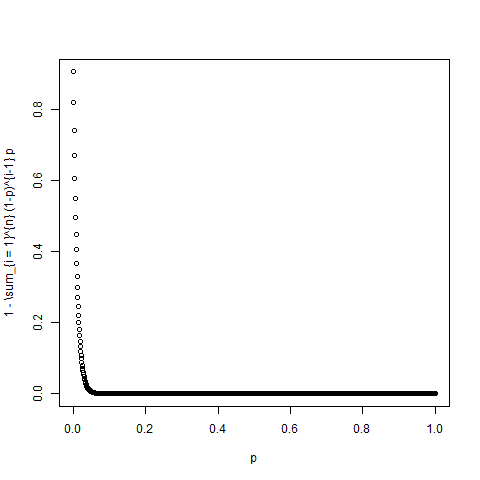
\includegraphics[width=6cm]{tarea2/problema2_1/graficas_inciso2_1_4/probabilidadDeQueC_pSupere100.png}
\end{center}\par\null

Con todo esto dicho, podemos garantizar que $C_p$ diverge a $\infty$ en distribución.\par\null

Entonces 
\begin{align}
    - \min_{n \leq C_p} \rightarrow - \min_{n \leq \infty} S_n = \min_{n \geq 0} S_n = M
\end{align}\par\null

Ahora recordemos que $g$ era una función continua y que $g>0$. Por lo tanto $1/g$ es una función continua,
con inverso derecho $f$ en $(0, 1)$. Es decir

Por lo tanto
\begin{align}
    \mw(M = n)  &=  \lim_{p \rightarrow 0} \mw(M_p = n)                         \\
                &=  \lim_{p \rightarrow 0} e^{-n f(1-p)}(1-e^{- f(1-p)})        \\
                &=   e^{-n f(1)}(1-e^{- f(1)}) \label{problema2_1:distribucion_de_M}
\end{align}

Lo cual corresponde a la distribución de una geométrica de parámetro $1-e^{- f(1)}$.\par\null

El caso donde $f(1^-) = 0$, implica que $\lim_{p\rightarrow0} (1-e^{- f(1-p)}) = 0$. El cual es complétamente
análogo al caso anterior donde considerábamos $p \rightarrow 0$ en geométricas de parámetro $p$.\par\null

Donde, habíamos dejado claro que conforme el parámetro disminuía hacia 0, las distribuciones de las geométricas divergía 
a la de $\infty$ y que por lo tanto la probabilidad de que nuestras geométricas tomaran cierto 
valor $n$ disminuía hacia $0$ conforme el parámetro tendía a $0$.\par\null

Incluso para este caso, la ecuación \eqref{problema2_1:distribucion_de_M} es válida según nuestro análisis, pues

\begin{align}
\mw(M = n)  &=  \lim_{p \rightarrow 0} \mw(M_p = n)                         \\
                &=  \lim_{p \rightarrow 0} e^{-n f(1-p)}(1-e^{- f(1-p)})    \\
                &=  e^{-n 0}(1-e^{- 0})                                     \\
                &=  1(1-1)                                                  \\
                &=  0.
\end{align}

Y esto, para toda $n \in \N$, justo como nuestro análisis de las distribuciones geométricas
nos dijo.
\end{proof}